\section{Background}
Metzler's and Westerhoff's model show that it is possible for endogenous business cycles to be induced through inventory cycles and the failure of firms to accurately predict future consumption. These models were designed to focus on the effects of firm expectations with Westerhoff's contribution consisting of introducing a heterogenous expectation rule that allows firms to switch behavior based on the state of the economy. Both of these models however simplify other aspects of the economy that feature more complex behavior in other business cycle models.

The inventory cycle model features 3 main factors of production: predicted consumption, investment, and inventory. Metzler and Westerhoff holds investment as an exogenously determined constant; however, this is both unrealistic and does not allow for long term endogenous growth. To incorporate a mechanism for endogenously adjusting investment, we take inspiration from the discrete time business cycle model described by T\"{o}nu Puu\autocite{Puu2003}. In order for investment to operate under Keynes' accelerator principle, capital stock must be in a proportion to the change in income, thus the investment level would be a function of the rate of change in income. 

A linear function for investment captures this premise; however, this leads to unrealistic behavior for higher magnitudes of income change. Suppose income dramatically increased; a linear function implies that a proportionally high level of investment can sustain this higher level of production when in reality other factors of production such as the land, labor, or technology available are the primary limiting factors. Of larger concern with a linear model though is if the economy encounters a sharp decrease in income. This induces a large, negative value for investment which implies that firms would actively destroy their machinery and other forms of capital stock in the event of an economic recession. This is obviously unrealistic and so John Hicks introduced a piecewise linear investment function such that at extreme levels of income change, investment will reach a predetermined maximal or minimal value. This piecewise function was then adapted to be differentiable over all points by Richard Goodwin by approximating the curve with a hyperbolic-tangent function\autocite{Puu2003}.

Puu approximates the hyperbolic-tangent function with its linear-cubic Taylor series expansion as this introduces a back-bending behavior into the curve. This allows the investment curve to capture not only firm behavior in the private sector but also implicitly include government spending and taxation. This follows from the now common policy for governments to engage in contracyclic behavior, increasing the quantity and size of spending projects and decreasing taxes when income is decreasing. Likewise, when the economy is performing well, the government cuts back on spending projects intended to stimulate the economy while also increasing taxes in order to take advantage of the overheating economy. 

The problem with the cubic function is that it leads to unbounded behavior in the extremes, much like the linear function. Puu resolves this by ensuring that income growth is bounded by [-1, 1]; this is not the case for our model however. We instead want a function that features similar curvature and behavior as the cubic function but flattens when income change is of significant magnitude. This can be accomplished with the following function:

\begin{equation}
    I_t = \frac{\frac{Y_{t-1}-Y_{t-2}}{v}}{(\frac{Y_{t-1}-Y_{t-2}}{v})^4+q}	
\end{equation}

The behavior of this function qualitatively resembles that of the linear-cubic function described in by Puu when $v,q>0$ and ; however, $\lim_{(Y_{t-1}-Y_{t-2})\to\infty}I_t=0$. This function is at its absolute maximum and minimum when:
\begin{equation*}
    Y_{t-1}-Y_{t-2}=\pm\frac{q^{1/4}v}{3^{1/4}}
\end{equation*}
Thus giving a maximal or minimal investment of:
\begin{equation*}
    I_t=\frac{3^{3/4}}{4q^{3/4}}
\end{equation*}
Intuitively, larger values of $v$ make the function "wider", increasing the range over $Y_{t-1}-Y_{t-2}$ where $I_t$ is not effectively 0. Smaller values of $q$ increases the magnitude of the maximum and minimum of the function, effectively making it taller. $v$ and $q$ cannot be directly attributed to any direct economic phenomena; however, their effect on the function can be interpreted analogously to the properties of the linear-cubic function. The "height" of the function determines the potential magnitude of investment and the "width" determines the rate at which investment, both private and public, react to changes in income.

Metzler describes the existence of two important lags in the study of Keynesian models. The Robertson lag is characterized by making current consumption a function of past income, i.e. consumption behavior lags behind current income. The Lundberg lag however concerns a discrepancy between the income level and the production decision of firms \autocite{Metzler1941} . These lags are named after the two economists D. H. Robertson and Erik Lundberg who developed models that contained only their eponymous lag type. Although both lags are likely to exist in reality, most models only incorporate one lag due to the increased complexity associated with it. Metzler and Westerhoff make use of a Lundberg lag by making income a function of the predicted level of consumption as opposed to actual consumption. T\"{o}nu Puu's model makes use of a Robertson in order to induce endogenous business cycles. Metzler himself does not claim that the Lundberg sequence is any more realistic than the Robertson sequence. Whichever lag has a longer time-period can be treated as of being greater importance but Metzler actually proposes a variety of scenarios that present contradicting conclusions. Suppose that decided their behavior on a quarterly basis but consumers altered their spending behavior with every paycheck, then it is no longer unrealistic to treat the Robertson lag as being of 0 length, i.e. nonexistent. If consumers revise their spending behavior every 6 months to a year, then it would actually be more realistic to include a non-zero Robertson lag while minimizing the Lundberg lag. 

For the purposes of this model, we will include a non-zero Lundberg and Robertson lag. The consumption function is treated exactly as presented in Puu:
\begin{equation}
    C_t=(1-s)Y_{t-1}+sY_{t-2}
\end{equation}
This function incorporates a 1-period Lundberg lag where $s\in[0,1]$ is the marginal propensity to save. This function also contains a 2-period delayed consumption due to the marginal propensity to save, thus all income made in some period $t$ can be though of as being eventually spent in the period $t+1$ and $t+2$. Although intuitive, this explanation is not wholly accurate as the Lundberg lag does not imply saving of income to spend in the next period but rather that spending behavior is influenced only on the information of lagged income level. The choice of $s$ dictates the relative importance of lagged income, a higher marginal propensity to save reduces the impact of income made in the previous time period but increases the effective impact of the income made two time periods ago.  

As the economy is also making use of a Robertson lag, income is not directly a function of consumption as may be seen in other models. Rather, income is viewed from a production standpoint. This is achieved by explicitly defining a predicted level of consumption. Westerhoff and Metzler use an equation similar to the form:

\begin{equation*} 
    U_t=C_{t-1}+\eta(C_{t-1}-C_{t-2})
\end{equation*}
However, this assumes that firms have no way to adapt their coefficient of expectation $\eta$. 

A new predictive mechanism requires that firms have bounded rationality. If firms possessed perfect rationality, then they would be able to perfectly predict consumption levels as consumption is based on lagged income, thus if we wish to maintain our Robertson lag, firms must still have bounded rationality. Another mechanism that firms can use that maintains better "memory" is that of an average. 
\begin{equation}\label{predict}
    U_t = \frac{C_{t-1}+C_{t-2}+C_{t-3}}{3}
\end{equation}
This formulation is an average of the consumption levels of the past 3 time periods. The choice of three time periods is relatively arbitrary and higher order difference equations of the same form can be used; however these higher order formulations can result in a less mathematically tractable model.

Inventory production proceeds as seen in Chapter 2 with firms producing $S_t$ explicitly to maintain Inventory at optimal levels:
\begin{equation}
    S_t = k U_t-Q_{t-1}
\end{equation}
where $Q_t$ is the level of inventory maintained at the end of time $t$ and $k\in[0,1]$. This can be solved for as the sum of the previous inventory level, production intended for inventory, and the difference between production intended for consumption and the actual consumption level:
\begin{equation}
    Q_t=Q_{t-1}+S_t+(U_t-C_t)
\end{equation}

Income level, or output, can thus be written as a sum of production:
\begin{equation}\label{eq:Income}
    Y_t=I_t+S_t+U_t
\end{equation}
However, as income has the capability of sustained growth under this model, it is preferable to analyze the rate of change of income in this model. In Appendix A, we show that the growth rate of the economy can be interpreted as a single variable, 6th order difference equation on $\dot Y$:
\begin{equation}
\begin{split}
    \dot Y_{t}& = \frac{\frac{\dot Y_{t-1}}{v}}{\left(\frac{\dot Y_{t-1}}{v}\right)^4+q}-\frac{\frac{\dot Y_{t-2}}{v}}{\left(\frac{\dot Y_{t-2}}{v}\right)^4+q} + \\
    & (1+k)\frac{(1-s)(\dot Y_{t-2}+\dot Y_{t-3}+\dot Y_{t-4})+s(\dot Y_{t-3}+\dot Y_{t-4}+\dot Y_{t-5})}{3} -\\
    &\left[(k+1)\frac{(1-s)(\dot Y_{t-3}+\dot Y_{t-4}+\dot Y_{t-5})+s(\dot Y_{t-4}+\dot Y_{t-5}+\dot Y_{t-6})}{3}\right.\\
    &\left.-(1-s)\dot Y_{t-2}-s\dot Y_{t-3}\right]
\end{split}
\end{equation}

\section{Growth Dynamics}
The long run dynamics of the model are highly dependent on the choice of initial conditions. Simulation of the model require a choice of 6 initial values of income change in addition to the parameter choice. If the 6 initial values are equivalent, all future iterations of the mapping are equal to this choice and the model remains in a stable steady state. It both more interesting and realistic then to consider cases where there is variation in initial income growth.
\begin{figure}[ht]
    \centering
    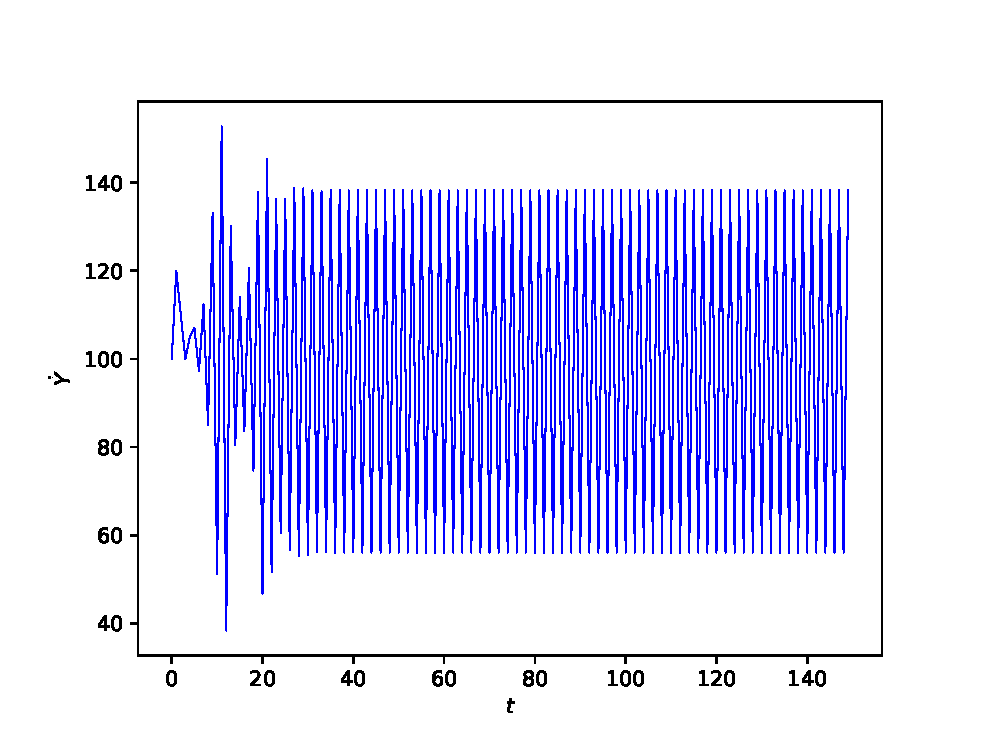
\includegraphics[height=0.4\textheight]{./metzlerian_growth/timeseries1.eps}
    \caption{Timeseries plot of income growth rate over 150 iterations. $s=0.6,\ k=0.3,\ v=500,\ q=0.001$. Initial values of $\dot Y$ are: 100, 120, 110, 100, 105, 107}
    \label{growth_timeseries1}
\end{figure}
Figure \ref{growth_timeseries1} displays a possible trajectory of income growth. Under the parameters listed, the trajectory clearly behaves in a stable, cyclic manner within 40 iterations. 

There do not exist techniques to solve generalized 6th order difference equations; however it is possible to computationally solve for the long run dynamics of the system.
\begin{figure}
    \centering
    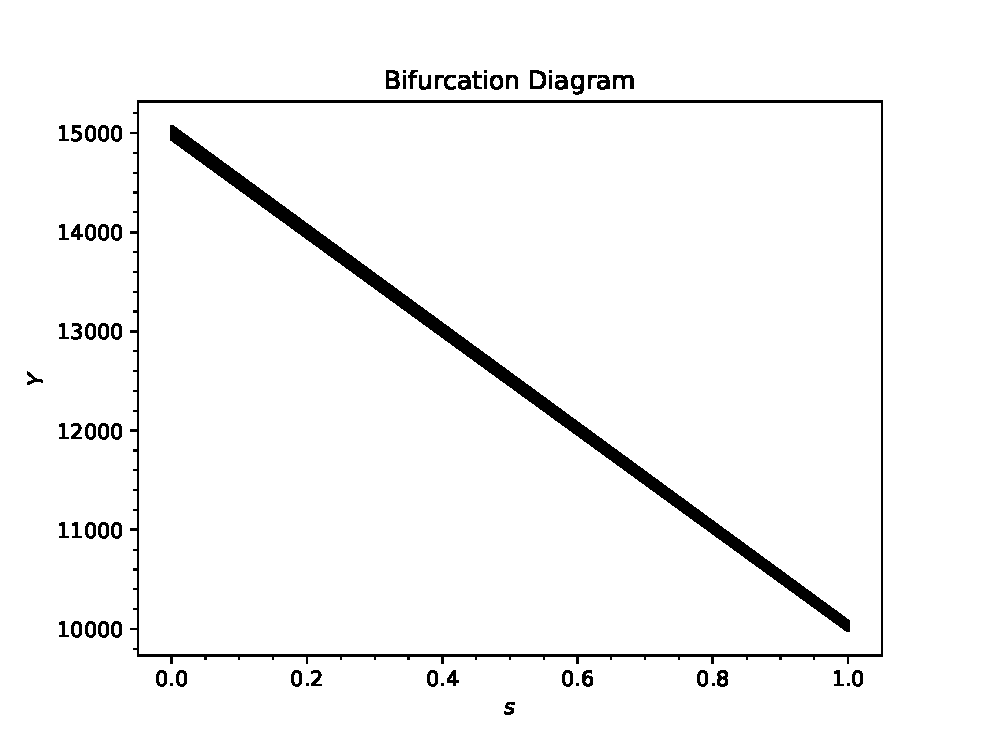
\includegraphics[height=0.4\textheight]{./metzlerian_growth/sbifurcation}
    \caption{Bifurcation diagram varying $s$ between 0.1 and 0.9. Initial conditions and other parameters are held constant as described in Figure \ref{growth_timeseries1}.}
    \label{metzlerian_growth-sbifurcation}
\end{figure}

The bifurcation diagram displayed in Figure \ref{metzlerian_growth-sbifurcation} displays the long-run behavior of the model as $s$ is varied. The methodology of the computational analysis and results are displayed in detail in Section \ref{bifurcation_analyzer} and Section \ref{bifurcation_analysis}, respectively. Long-run values are rounded to their nearest whole number for the purposes of this computational analysis although it is possible to account for higher levels of numerical precision using the analyzer. A bifurcation point exists at $s=0.65$ and $s=0.53$, the mapping is a stable 2 cycle when $s$ is between these two values. 

\begin{figure}
    \centering
    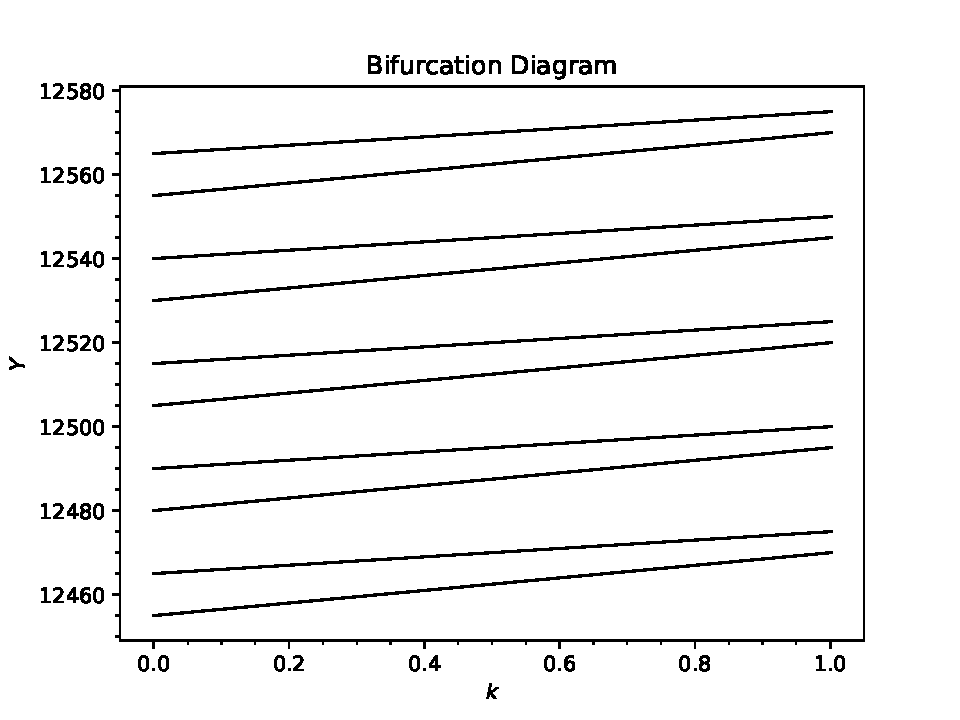
\includegraphics[height=0.4\textheight]{./metzlerian_growth/kbifurcation}
    \caption{Bifurcation diagram varying $k$ between 0.1 and 0.9. Initial conditions and other parameters are held constant as described in Figure \ref{growth_timeseries1}.}
    \label{metzlerian_growth-kbifurcation}
\end{figure}

The bifurcation diagram varying $k$ qualitatively appears much simpler than Figure \ref{metzlerian_growth-sbifurcation}. This diagram displays stable, 2-cycle behavior except when $\leq k$










